%\documentclass{article}
%\usepackage[a4paper, total={6in, 8in}]{geometry}
\documentclass[reprint,amsmath,amssymb,rmp,onecolumn,notitlepage,11pt]{revtex4-1}
\usepackage[utf8]{inputenc}
%\usepackage{authblk}
%\usepackage{natbib}
\usepackage[normalem]{ulem}
\usepackage{graphicx}
\usepackage{hyperref}
\usepackage{xcolor}
\newcommand{\red}[1]{\textcolor{red!80!black}{#1}}
\newcommand{\blue}[1]{\textcolor{blue!80!black}{#1}}
\newcommand{\green}[1]{\textcolor{green!70!black}{#1}}
\usepackage{mathtools}
\DeclarePairedDelimiter{\evdel}{\langle}{\rangle}
\usepackage[colorinlistoftodos]{todonotes}

\begin{document}
\title{The role of geometry in the chain separation distribution of links in protein contact networks}
%\title{}
%\title{}
%\title{}
\author{Nora Molkenthin}
\email[Electronic Address: ]{n.molkenthin@gmx.de}
\affiliation{Potsdam Institut für Klimafolgenforschung, Potsdam, Germany}
\affiliation{Chair for Network Dynamics, Institute for Theoretical Physics and Center for Advancing Electronics Dresden (cfaed), Technical University of Dresden, 01069 Dresden}
\author{Antonia S J S Mey}
\affiliation{EaStCHEM School of Chemistry, University of Edinburgh, Edinburgh, United Kingdom}
\author{Steffen Mühle}
\affiliation{Uni Göttingen, 37077 Göttingen, Germany}

%\author{Marc Timme}
% \affiliation{Network Dynamics, Max Planck Institute for Dynamics and Self-Organization (MPIDS), 37077 Göttingen, Germany}
% \affiliation{Chair for Network Dynamics, Institute for Theoretical Physics and Center for Advancing Electronics Dresden (cfaed), Technical University of Dresden, 01069 Dresden}

\begin{abstract}
The distribution of chain separations of interacting amino acids in proteins roughly follows a power law. Here we show, analytically and in simulations, that a geometrical stochastic model of folding chains can explain this behaviour. %Separating the data in $\alpha$-dominated, $\beta$-dominated and intrinsically disordered proteins (IDP's) shows characteristic structures in the distribution due to the secondary structure.
\end{abstract}
\maketitle

\section*{Introduction}
Proteins, the molecular machines of every living organism perform vital tasks required for life to persist, ranging from transport (e.g. hemoglobin), signal transduction (e.g. rhodopsin), immune responses (e.g. antibodies), and hormonal regulation (e.g. insulin)~\cite{}. All natural proteins are made up of 20 different amino acids which dictate the three dimensional conformations the proteins adopt in order to function~\cite{}. One way of looking at the functional forms of proteins and classifying their structural properties is by looking at protein residue or contact networks~\cite{Vendruscolo2002,DiPaola2013,Estrada2011}. Protein Contact Networks (PCN), have shown promise in understanding protein folding patterns as well as revealing allosteric communication pathways~\cite{https://pubs.acs.org/doi/10.1021/acs.jcim.9b00320, and others}. 
Prom a physicist perspective it is interesting to understand the emergent behaviour in protein structure from PCNs, by investigating common network measures and their behaviour for PCNs. For example Bartoli et al. observe that proteins have a sequence separation distribution that follows $\frac{1}{\ell}$, where $\ell$ is the separation of two connected amino acids along the backbone chain. However, they do not provide an explanation for this observation~\cite{bartoli2008effect}. 
Here, we will show how a simple geometrical model can capture this behaviour well, even providing a simple analytical approximation. The analytical approximation and geometrical model build on the idea that inherently geometrical objects, such as amino acids, imply that any resulting PCN network ensemble modelling them has to be spatially embedded~\cite{}. 
Different approaches have been used in the past for geometrical models describing protein folding, some of which derived characteristics of the secondary structure from constraints on bond and torsion angles~\cite{Danielsson2010,Molkenthin2011} and others focused on the formation mechanisms of the tertiary structure~\cite{molkenthin2016scaling, molkenthin2020self}. Based on such considerations, we have constructed a network formation process, in which random connections are added to a chain of unit disks, without causing them to intersect~\cite{molkenthin2016scaling}. Such a model can now be used to investigate the emergenct behaviour of sequence separation distributions as observed by Bartoli et al.~\cite{bartoli2008effect}. To this end, we analyze the sequence separation distribution that emerge from the geometric model, where the length $\ell$ of a link is defined as the distance of the two ends along the original chain.
This is then compared to the sequence separation distribution extracted from protein residue networks (PRN) generated from protein data bank data. 

\todo[inline, color={green!40}]{@Nora: Summary of our findings and why this is cool.}


\section*{Protein Residue Networks and their synthetic counterparts}
The complex interaction pattern between the amino acids in a protein can be very naturally expressed as a network, in which each amino acid is represented by a node and spatial proximity is encoded as a link. Whenever two central $C_\alpha$ atoms are closer together than a threshold $d_c$, they are connected. These connections are encoded in the adjacency matrix of the folded protein, which is the binary matrix
\begin{equation}
  A^{\textsf{PDB}}_{ij}=
  \begin{cases}
   0, & \text{ if } d_{i,j}>d_c \text{ or } i=j\\
      1, & \text{ if } d_{i,j}\leq d_c .
      \end{cases}
    \label{eq:aij}
\end{equation}
Adjacency matrices are commonly used to describe networks and in this case represent the PRN.

The underlying formation mechanisms of individual protein folds are incredibly complex and depend on the surrounding solvent as well as the specific amino acid sequence and their quantum-mechanical interactions. Here we want to study the ensemble of all proteins, however, and will thus "average out" such specifics.

Based on the basic assumption that amino acids are objects in space, that can not overlap indefinitely, we introduced a model in \cite{molkenthin2020self} starting from a chain of identical spheres, each in contact only with the neighbours it is connected to. Then additional connections form by randomly selecting two spheres and moving them towards each other until they touch, the new links formed that way can not be broken in later steps and function as constraints on subsequent links. If contact of the two selected spheres is geometrically impossible without breaking previously made connections or leading to overlaps of any spheres, the link is not made and taken out of the pool of possible connections. This process is repeated until no more links can be formed without violating the geometric constraints.

In \cite{molkenthin2016scaling}, we have introduced a simplified, two-dimensional version of this model, which starts from a closed chain of $N$ unit discs and subsequently adds links, such that connected discs touch, yet no discs intersect. The advantage of this model is, that it can be approximated by a purely topological simplification, which can be treated analytically.

The topological constraints in the resulting network model are:
(a) New links always form between two units that are part of the same face of the graph (region enclosed by a cycle in the network). This prevents the overlapping of discs. (b) No links form across the outer face. This prevents the enclosure of a unit by less than six other units (which is geometrically impossible) such that. (c) The maximum degree of each unit is six, as six is the maximum number of unit discs, one central unit disc can touch. (d) Once connected by a link, pairs of units do not disconnect.

\section*{Analytic approximation}
Here we want to analytically approximate the sequence separation distribution for the simplified 2D model, that is the separation along the backbone chain of two nodes connected by a link, as illustrated in Fig~\ref{fig:fig_prn_vis}.
\begin{figure}[h]
    \centering
    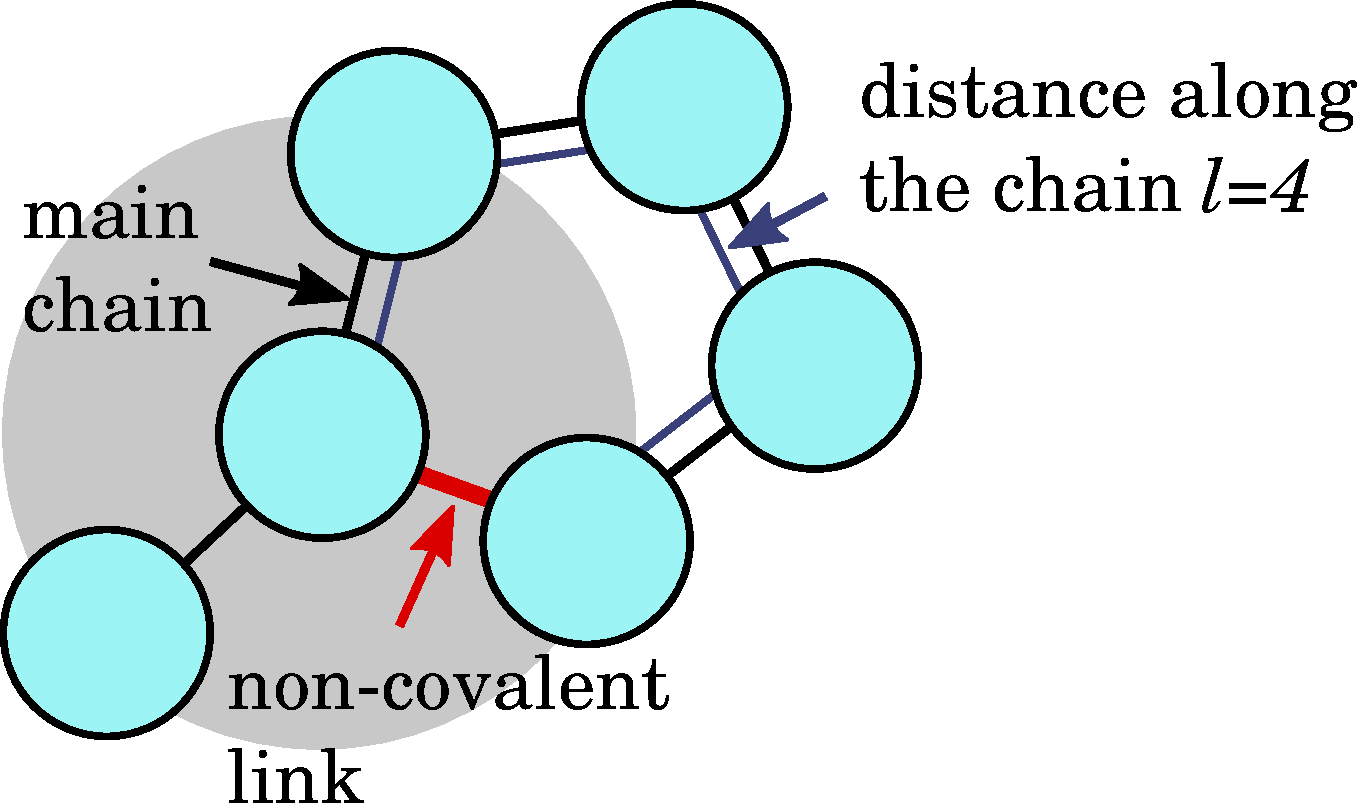
\includegraphics[width=0.3\columnwidth]{figures/prn_vis.pdf}
    \caption{The sequence separation distribution is defined as the separation along the chain (blue) of two connected units (red).}
    \label{fig:fig_prn_vis}
\end{figure}

Let us start by introducing the auxiliary variable $F(s)$, defined to be the number of possible links with a sequence separation of $s$. Before any links are added all sequence separations are equally likely, as there are $N$ possibilities of making a link of each separation $s$ with $2\leq s < N/2$.

As we add more links, not only are links taken out of this pool, because they have already been realized, each existing link can also geometrically prohibit other connections.
Let us call the pools of available links after $i$ links have been added $F_i(s)$.
\\

\red{----------- Add Figure explaining which links are geometrically excluded, maybe include in fig 1 -----------}
\\

The expected distribution of possible links after one step is given by the average over available link pools taken over all possible lengths of the initial link
\begin{equation}
    F_1(s)= \frac{1}{N/2-2} \sum_{s_1=2}^{N/2} { \begin{cases}
    N-2(s-1) \text{ , for } s<s_1\\
    N-2(s_1 -1)\text{ , for } s\geq s_1
    \end{cases}}.
\end{equation}

In subsequent steps we get the same reduction but starting from the pool of the step before rather than the full $N$ links for each length, leading to an additional probability factor \red{explain this in more detail, I already forgot exactly why that is...}
\begin{equation}
    P_k(s)=\frac{F_k(s)}{C_k},
    \label{eq.Pk}
\end{equation}
with $C_k=\sum_{s=2}^{N/2}F^k(s)$, for each segment separation $s$ to occur and thus
\begin{equation}
    F_k(s)= \frac{1}{N/2-2} \sum_{s_k=2}^{N/2} {\begin{cases}
     F_{k-1}(s)-2(s-1) P_k(s) \text{ , for } s<s_k\\
     F_{k-1}(s)-2(s_k -1)P_k(s)\text{ , for } s\geq s_k
    \end{cases}}.
\end{equation}
This can be simplified to
\begin{align}
   F_k(s)&= \frac{1}{\frac{N}{2}-2} \frac{F_{k-1}(s)}{C_{k-1}}\left( \sum_{s_k=2}^{N/2}C_{k-1} - \sum_{s_k=2}^{s} 2(s_k-1) - \sum_{s_k=s+1}^{N/2} 2(s -1) \right) \nonumber \\
   &= \frac{1}{\frac{N}{2}-2}\frac{F_{k-1}(s)}{C_{k-1}}\left(\left(\frac{N}{2}-2\right)C_{k-1} -(s^2-s)-2\left(\frac{N}{2}-(s+1)\right)(s-1)\right)  \nonumber \\
   &= F_{k-1}(s)\left(1-\frac{-s^2 +(N-1)s-(N+1)}{(\frac{N}{2}-2)C_{k-1}} \right)\nonumber \\
   &=F_{k-1}(s)\left(1-\frac{f(s)}{(\frac{N}{2}-2)C_{k-1}} \right)
   \label{eq.Fk_rec}
\end{align}
Where we defined $f(s)=-s^2 +(N-1)s-(N+1) \approx N s - s^2 - N$ for notational brevity.

We can now use the recursive expression Eq.~\ref{eq.Fk_rec} to write down a closed expression for $F_k(s)$

\begin{equation}
    F_k(s)=N\prod_{i}^k\left(1-\frac{f(s)}{(\frac{N}{2}-2)C_{i-1}} \right)
\end{equation}

The probability distribution of the realized sequence separations of all added links is then given by the average over the available pools at each link addition step, leading to
\begin{align}
    P(s)&=\frac{1}{N-3}\sum_{k=0}^{N-3} P_k(s) \nonumber \\
    &= \frac{N}{N-3}\sum_{k=0}^{N-3} \frac{1}{C_k}\prod_{i}^k\left(1-\frac{f(s)}{(\frac{N}{2}-2)C_{i-1}} \right),
\end{align}
which makes use of Eq.~\ref{eq.Pk}. The only unknown in this expression is $C_k$, which we can not compute exactly. However, since $C_k$ monotonically decreases with $k$, $N>C_k>C_{N-2}$ always holds and we can obtain an upper and lower bound by replacing all $C_k$ in the expression with either $N$ (underestimates all probabilities) or $C_{N-2}$ (overestimates all probabilities). Each time we get an expression of the form 
\begin{align}
     P(s)&\approx\frac{N}{N-3}\sum_{k=0}^{N-3} \frac{1}{C_k}\prod_{i}^k\left(1-\frac{f(s)}{(\frac{N}{2}-2)C} \right)\nonumber \\
     &=\frac{N}{N-3} \sum_{k=0}^{N-3}\frac{1}{C_k}\left(1-\frac{f(s)}{(\frac{N}{2}-2)C} \right)^k \nonumber \\
     &\approx \frac{A}{f(s)}
\end{align}
for $1<s<\frac{N}{2}$,
where $A$ is an unknown constant, containing an approximation of the various normalization constants $C_i$, as well as the direct effects of the chain length. 
Since for long chains, $f(s)$ is largely dominated by the linear term, the distribution is well approximated by a power law with an exponent of $-1$. We have made use of the geometric series to approximately find a closed solution. 

In the last step of this approximation, we take the $C_k$ to all be approximately equal in order to apply the geometric series. However, in reality we know $1/C_k$ to increase with $k$, giving large $k$ summands relatively more weight than in a geometric series. This would lead to a correction in the exponent.

\begin{equation}
    P_{corrected}(s)\approx A f(s)^{-1+\alpha},
\end{equation}
where $0<\alpha<1$ \red{why cant $\alpha$ be >1?}.


\section*{Data and simulations}
 For large values of the chain length $N$ we thus find an approximate power law probability distribution for the sequence separation with an exponent of -1 \red{include note of correction}. Here we use simulations, as introduced in \cite{molkenthin2020self} and networks extracted from measured protein data from the PDB \cite{PDB} to compare this behaviour in realistic 3D settings and show that the basic principle persists, indicating that the sequence distance separation distribution is largely determined by simple geometric constraints.
 

\begin{figure}[h]
        \centering
	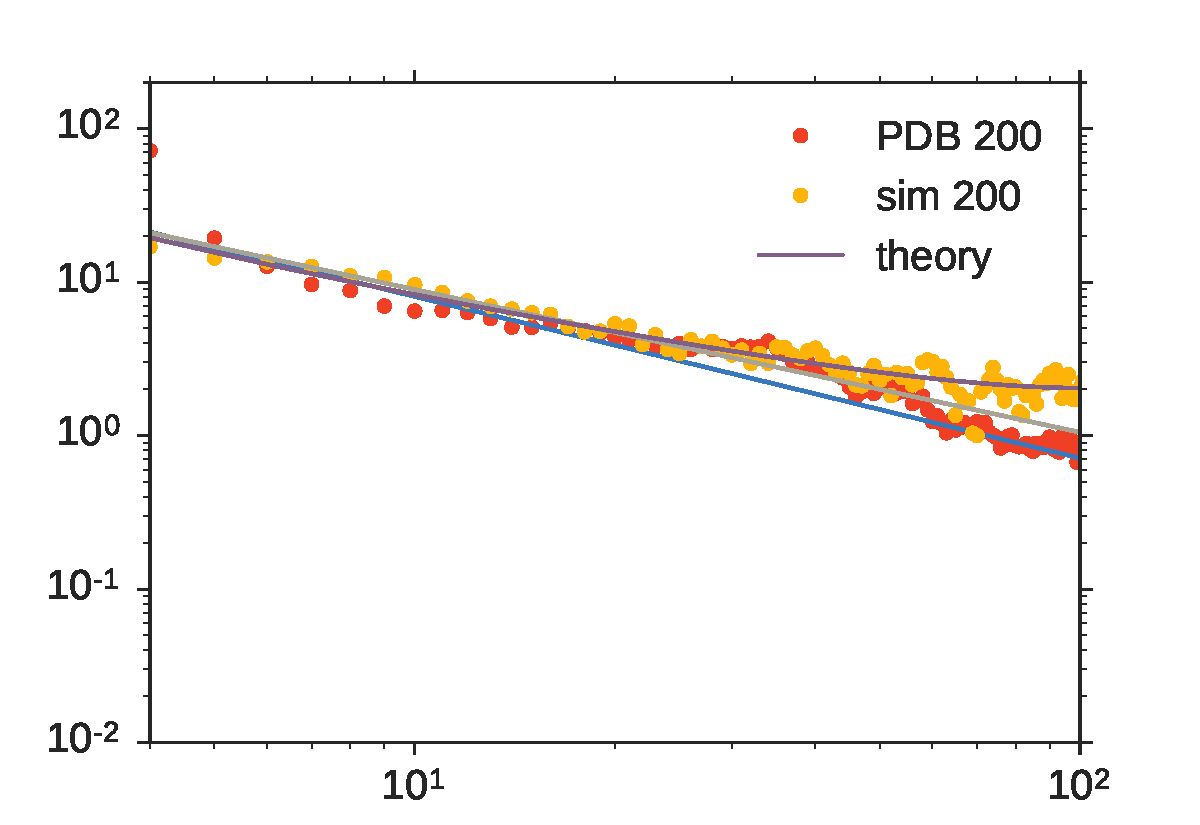
\includegraphics[width=0.45\textwidth]{figures/both_200.pdf}
	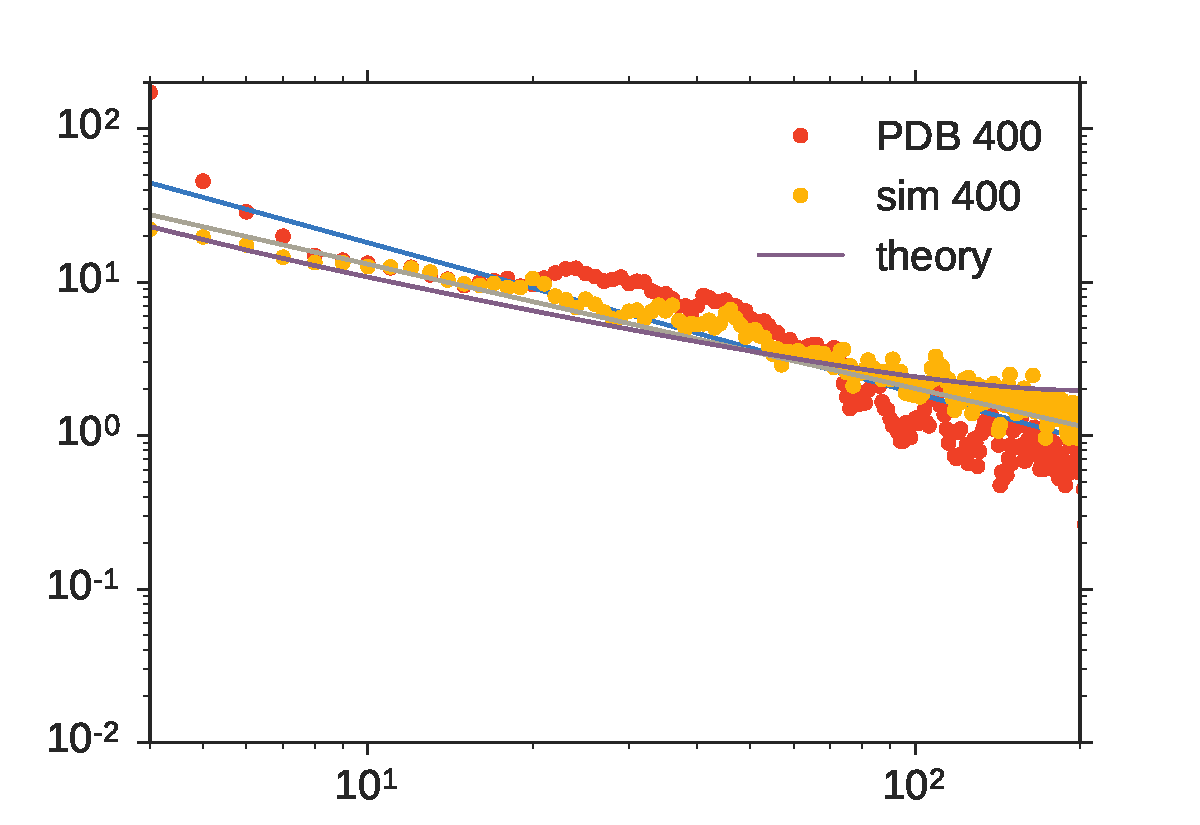
\includegraphics[width=0.45\textwidth]{figures/both_400.pdf}
        \caption{Sequence distance distributions for real and simulated folds for a) Chain lengths around 200 b) chain lengths around 400. The theoretical curve for 2D rings works okay for 3D open chains (because the rings are closed sequence separations of more than N/2 are a bit meaningless and thus not accounted for) The parameters used in this are $A=80$ and $\alpha=0.2$ in a) and $0.3$ in b). I thought in b) it makes sense for $\alpha$ to be larger as there are even larger exponents $k$ coming into relevance. I'm not sure we want to use that whole $\alpha$ argument too much though as it's a but ad-hoc and would be nicer to just fit $A$ and be done with it, but then it may look a bit more off.
        }
        \label{fig:time_scaling}
\end{figure}
\red{We observe that, while the general shape seems to match, in real proteins sequence separations of 20 to 60 amino acids are slightly over represented. We need to comment on that somehow. Also links of length 2 and 3 are over represented, we need to discuss that too.}

\red{To check if the bump has something to do with the secondary structure that is present in real proteins but not in the model, we have generated a sample of intrinsically disordered proteins, that also do not contain secondary structures. The bump does indeed disappear. The over representation of 2 and 3 does not though and there os probably a simple explanation for that and maybe we can simply take those points out and redo the mean degree matching and get to lines that are not just parallel but actually on top of one another that way.}
\begin{figure}[h]
        \centering
	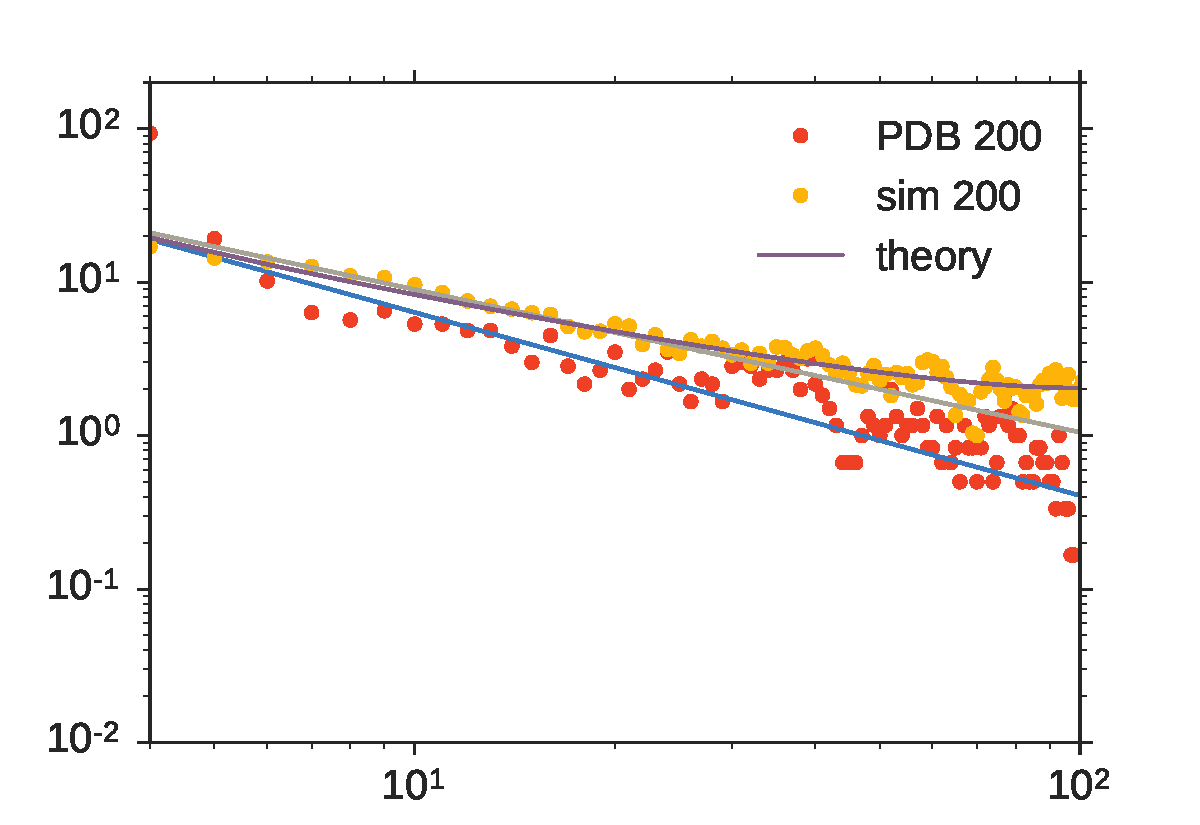
\includegraphics[width=0.45\textwidth]{figures/idp_200.pdf}
	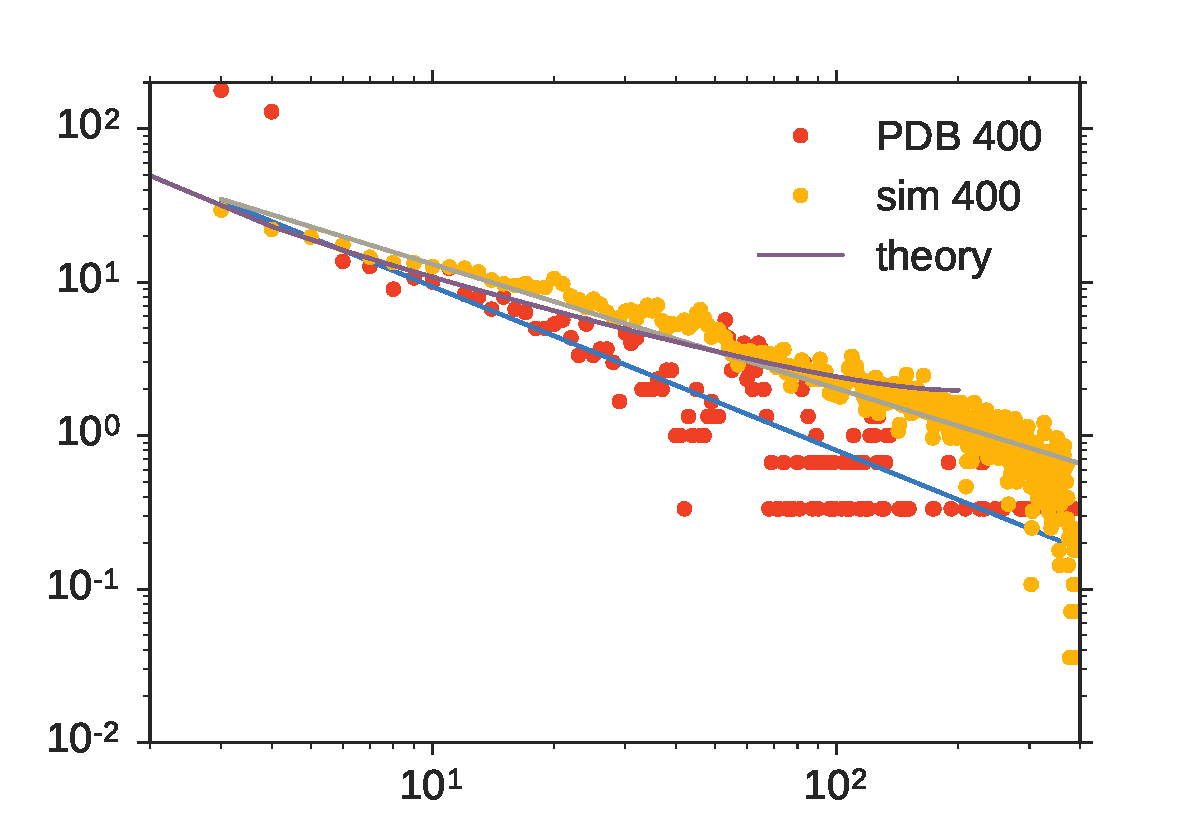
\includegraphics[width=0.45\textwidth]{figures/idp_400.pdf}
        \caption{Sequence distance distributions for intrinsically disordered proteins and simulated folds for a) Chain lengths around 200 b) chain lengths around 400. The theoretical curve for 2D rings works okay for 3D open chains (because the rings are closed sequence separations of more than N/2 are a bit meaningless and thus not accounted for) The parameters used in this are $A=80$ and $\alpha=0.2$ in a) and $0.3$ in b). I thought in b) it makes sense for $\alpha$ to be larger as there are even larger exponents $k$ coming into relevance. I'm not sure we want to use that whole $\alpha$ argument too much though as it's a but ad-hoc and would be nicer to just fit $A$ and be done with it, but then it may look a bit more off.
        }
        \label{fig:time_scaling}
\end{figure}
\section*{Conclusion}
\begin{enumerate}
    \item We can now explain the sequence separation from geometry and even do it analytically.
    \item Maybe something about helixes and sheets and the dip.
\end{enumerate}
TO DO: Leave until the rest is done.
\section*{Declarations}
\subsection{Availability of data and materials}
All data generated or analysed during this study are included in this published article [and its supplementary information files].
\subsection{Competing interests}
The authors declare no competing interests.
\subsection{Funding}
This research was supported by ...
\subsection{Authors' contributions}

\subsection{Acknowledgements}
We thank ... for fruitful discussions.

\bibliographystyle{unsrt}
\bibliography{proteins}

\appendix
\section{Supplemental Material Collection}
\section{Random ideas}
\begin{itemize}
    \item Why is the beginning different for simulations?
    \item Does the dip disappear for IDPs
    \item Can we use all NMR structures for IDPs
    \item Would it help using more simulated structures than just the Crystal structure. 
\end{itemize}



\end{document}